% --------------------------------------------------
%  TALLER DE INTRODUCCIÓN A LaTeX
%  https://github.com/mianfg/latex-intro
%
%  Sesión 1 -> Presentación
%
%  Autor: Miguel Ángel Fernández Gutiérrez, @mianfg
%  Fecha: 20 febrero, 2019
% --------------------------------------------------

% Tipo de documento (presentación)
\documentclass[10pt, xcolor=table]{beamer}
\usepackage{caption}
\usepackage{subcaption}

% Cargar el tema
\usetheme{metropolis}

%  __________
% |          |
% | Paquetes |
% |__________|

% Paquetes de idioma
\usepackage[utf8]{inputenc}
\usepackage[spanish, es-tabla, es-lcroman, es-noquoting]{babel}

% Paquete para código fuente
% LISTINGS
\usepackage{listings}
\usepackage{lipsum}
\usepackage{courier}
\usepackage{csvsimple}

% Colores para los bloques de código
\definecolor{codegreen}{rgb}{0,0.6,0}
\definecolor{codegray}{rgb}{0.5,0.5,0.5}
\definecolor{codepurple}{rgb}{0.58,0,0.82}
\definecolor{backcolour}{rgb}{0.95,0.95,0.92}
\lstdefinestyle{mystyle}{
	backgroundcolor=\color{backcolour},   
	commentstyle=\color{codegreen},
	keywordstyle=\color{blue},
	numberstyle=\tiny\color{codegray},
	stringstyle=\color{codepurple},
	basicstyle=\footnotesize\ttfamily,
	breakatwhitespace=false,         
	breaklines=true,                 
	captionpos=b,                    
	keepspaces=true,                 
	numbers=left,                    
	numbersep=5pt,                  
	showspaces=false,                
	showstringspaces=false,
	showtabs=false,                  
	tabsize=4
}
\lstset{style=mystyle}

% Paquete de numeración en Beamer
\usepackage{appendixnumberbeamer}

% Paquete de uso para plantilla
\usepackage{booktabs}
\usepackage[scale=2]{ccicons}

% Paquete para controlar espacios
\usepackage{xspace}
\newcommand{\themename}{\textbf{\textsc{metropolis}}\xspace}

% Paquetes para matemáticas
\usepackage{amsmath}    % Paquete básico de matemáticas
\usepackage{amsthm}     % Teoremas
\usepackage{mathrsfs}   % Fuente para ciertas letras utilizadas en matemáticas

% Paquetes para fuentes
\usepackage{newpxtext, newpxmath}   % Fuente similar a Palatino
\usepackage{FiraSans}               % Fuente sans serif
\usepackage[T1]{fontenc}
\usepackage[italic]{mathastext}     % Utiliza la fuente del documento
                                    % en los entornos matemáticos

%  ________________________
% |                        |
% | Configuración del tema |
% |________________________|

% Configuración básica del tema
\metroset{
  % tema oscuro ('dark') o claro ('light'). No tiene efecto al usar la
  % paleta de colores más adelante
  background=light,
  % 'none' para eliminar la diapositiva inicial de cada sección
  sectionpage=progressbar,
  % 'progressbar' o 'simple' para añadir una diapositiva inicial a cada subsección
  subsectionpage=none,
  % contador de página: 'none', 'counter' o 'fraction'
  numbering=none,
  % barra de progreso: 'none', 'head', 'frametitle' o 'foot'
  progressbar=frametitle,
  % fondo de los bloques estilo teorema: 'transparent' o 'fill'
  block=fill,
}

% Paleta de colores
\definecolor{accent}{HTML}{009688}
\colorlet{darkaccent}{accent!70!black}
\definecolor{foreground}{RGB}{0, 0, 0}
\definecolor{background}{RGB}{255, 255, 255}

% Insertar los colores en el tema
\setbeamercolor{normal text}{fg=foreground, bg=background}
\setbeamercolor{alerted text}{fg=darkaccent, bg=background}
\setbeamercolor{example text}{fg=foreground, bg=background}
\setbeamercolor{frametitle}{fg=background, bg=accent}

\setbeamercolor{headtitle}{fg=background!70!accent,bg=accent!90!foreground}
\setbeamercolor{headnav}{fg=background,bg=accent!90!foreground}
\setbeamercolor{section in head/foot}{fg=background,bg=accent}

\defbeamertemplate*{headline}{miniframes theme no subsection}{
  % Caja para mostrar título y autor encima de cada diapositiva
  % Nosotros no 
  %% \begin{beamercolorbox}[ht=2.5ex,dp=1.125ex,
  %%     leftskip=.3cm,rightskip=.3cm plus1fil]{headtitle}
  %%   {\usebeamerfont{title in head/foot}\insertshorttitle}
  %%   \hfill
  %%   \leavevmode{\usebeamerfont{author in head/foot}\insertshortauthor}
  %% \end{beamercolorbox}
  %% \begin{beamercolorbox}[colsep=1.5pt]{upper separation line head}
  %% \end{beamercolorbox}

  % Caja para mostrar navegación encima de cada diapositiva
  \begin{beamercolorbox}{headnav}
    \vskip2pt\insertnavigation{\paperwidth}\vskip2pt
  \end{beamercolorbox}
  \begin{beamercolorbox}[colsep=1.5pt]{lower separation line head}
  \end{beamercolorbox}
}

%  _________
% |         |
% | Ajustes |
% |_________|

% Fijar tabla a posición
\usepackage{array}
\newcolumntype{L}[1]{>{\raggedright\let\newline\\\arraybackslash\hspace{0pt}}m{#1}}
\newcolumntype{C}[1]{>{\centering\let\newline\\\arraybackslash\hspace{0pt}}m{#1}}
\newcolumntype{R}[1]{>{\raggedleft\let\newline\\\arraybackslash\hspace{0pt}}m{#1}}

%  ________
% |        |
% | Título |
% |________|

\title{Análisis de eficiencia de algoritmos}
\subtitle{Algorítmica. \alert{Práctica 1}}
\date{}
\author{Jose Alberto Hoces Castro\\Javier Gómez López\\Moya Martín Castaño\\[4pt]}
\titlegraphic{\hfill
\includegraphics[width=2.5cm]{logo_dark.jpg}}

%  ___________
% |           |
% | Documento |
% |___________|

\begin{document}
\maketitle

\begin{frame}{Contenidos}
	\setbeamertemplate{section in toc}[sections numbered]
	\tableofcontents[]
\end{frame}

\section{Introducción}
\begin{frame}[fragile]{Análisis de eficiencia de algoritmos}
	\begin{itemize}
		\item \textbf{Análisis de la eficiencia teórica:} estudio de la complejidad teórica de algoritmos.
		\item \textbf{Análisis de la eficiencia empírica:} ejecución y medición de tiempos de ejecución de los algoritmos estudiados.
		\item \textbf{Análisis de la eficiencia híbrida:} obtención de las constantes ocultas.
	\end{itemize}
\end{frame}

\begin{frame}[fragile]{Cálculo de la eficiencia teórica}
Consiste en analizar sobre el papel el peor tiempo de ejecución posible en un algoritmo para decidir en qué clase de funciones en notación \(\mathcal{O}\) se encuentra
\end{frame}

\begin{frame}[fragile]{Cálculo de la eficiencia empírica}
Ejecución de los algortimos en distintos agentes tecnológicos, calculando su tiempo de ejecución con la librería \texttt{<chrono>}.
\end{frame}

\begin{frame}[fragile]{Cálculo de la eficiencia híbrida}
Obtención de las constantes ocultas a través de gnuplot.
\end{frame}

\section{Análisis de los algoritmos propuestos}

\begin{frame}[fragile]{Algoritmos trabajados}
Se ha realizado un análisis de los siguientes algoritmos:
\begin{enumerate}
	\item Algoritmo de Inserción
	\item Algoritmo de Selección
	\item Algoritmo de Quicksort
	\item Algoritmo de Heapsort
	\item Algoritmo de Floyd
	\item Algoritmos de las torres de Hanoi
\end{enumerate}
\end{frame}


\begin{frame}[fragile]{Inserción}
	El código del algoritmo de Inserción es el siguiente:
	\lstinputlisting[language=C++]{./Codes/insercion.cpp}
\end{frame}

\begin{frame}[fragile]{Inserción.
		\normalfont{Eficiencia teórica}}
	En los comentarios del código observamos el análisis de la función.
	
	Son dos bucles, uno \texttt{for} y otro \texttt{while}, los cuales están anidados y por ser cada uno \(\mathcal{O}(n)\):
	\[
	T(n) \in \mathcal{O}(n^2)
	\]
\end{frame}

\begin{frame}[fragile]{Inserción.
		\normalfont{Eficiencia empírica}}
	\begin{table}[h!]
		\centering
		\footnotesize
		\scalebox{0.6}{
			\begin{tabular}{|c|c|}
				\hline
				\multicolumn{2}{|c|}{\textsf{Intel Core i7-6700 3.40 GHz}}
				\\\hline
				\bfseries Elementos (n) & \bfseries Tiempo (s)
				\csvreader{./data/Javi5454/salida_insercion.csv}{}
				{\\\hline\csvcoli&\csvcolii}
				\\\hline
			\end{tabular}
		}
		\scalebox{0.6}{
			\begin{tabular}{|c|c|}
				\hline
				\multicolumn{2}{|c|}{\textsf{i5-1095G1 1.00 GHz}}
				\\\hline
				\bfseries Elementos (n) & \bfseries Tiempo (s)
				\csvreader{./data/Jota/salida_insercion.csv}{}
				{\\\hline\csvcoli&\csvcolii}
				\\\hline
			\end{tabular}
		}
		\scalebox{0.6}{
			\begin{tabular}{|c|c|}
				\hline
				\multicolumn{2}{|c|}{\textsf{Ordenador Moya}}
				\\\hline
				\bfseries Elementos (n) & \bfseries Tiempo (s)
				\csvreader{./data/Moya/salida_insercion.csv}{}
				{\\\hline\csvcoli&\csvcolii}
				\\\hline
			\end{tabular}
		}
		\caption{Experiencia empírica de algoritmo de Inserción sin optimizar}
	\end{table}
\end{frame}

\begin{frame}[fragile]{Inserción.
		\normalfont{Eficiencia híbrida}}
	\centering
	\includegraphics[scale=0.15]{../../Images/Inserción combinados.png}
\end{frame}

\begin{frame}[fragile]{Inserción.
		\normalfont{Eficiencia híbrida}}
	\begin{itemize}
		\item i7-6700 3.40Ghz \(\rightarrow T_1(n) = 8.49924 \cdot 10^{-10} x^2 - 8.57879 \cdot 10^{-6} x + 0.546581\).
		\item Ordenador José Alberto \(\rightarrow T_2(n) = 7.96341 \cdot 10^{-10} x^2 + 2.23563 \cdot 10^{-5} x - 0.592279\).
		\item Ordenador Manuel \(\rightarrow T_3(n) = 1.04394 \cdot 10^{-9} x^2 + 1.58593 \cdot 10^{-6} x - 0.0969414\).
	\end{itemize}
	
	Varianza residual:
	\begin{itemize}
		\item \(T_1(n) \longrightarrow Var.res = 0.00162352\)
		\item \(T_2(n) \longrightarrow Var.res = 0.0050675\)
		\item \(T_3(n) \longrightarrow Var.res = 0.00161535\)
	\end{itemize}
\end{frame}

\begin{frame}[fragile]{Selección}
	El código del algoritmo de Selección es el siguiente:
	\lstinputlisting[language=C++]{./Codes/seleccion.cpp}
\end{frame}

\begin{frame}[fragile]{Selección.
		\normalfont{Eficiencia teórica}}
	En los comentarios del código observamos el análisis de la función.
	
	Son dos bucles \texttt{for}, los cuales están anidados y por ser cada uno \(\mathcal{O}(n)\):
	\[
	T(n) \in \mathcal{O}(n^2)
	\]
\end{frame}

\begin{frame}[fragile]{Selección.
		\normalfont{Eficiencia empírica}}
	\begin{table}[h!]
		\centering
		\footnotesize
		\scalebox{0.6}{
			\begin{tabular}{|c|c|}
				\hline
				\multicolumn{2}{|c|}{\textsf{Intel Core i7-6700 3.40 GHz}}
				\\\hline
				\bfseries Elementos (n) & \bfseries Tiempo (s)
				\csvreader{./data/Javi5454/salida_seleccion.csv}{}
				{\\\hline\csvcoli&\csvcolii}
				\\\hline
			\end{tabular}
		}
		\scalebox{0.6}{
			\begin{tabular}{|c|c|}
				\hline
				\multicolumn{2}{|c|}{\textsf{i5-1095G1 1.00 GHz}}
				\\\hline
				\bfseries Elementos (n) & \bfseries Tiempo (s)
				\csvreader{./data/Jota/salida_seleccion.csv}{}
				{\\\hline\csvcoli&\csvcolii}
				\\\hline
			\end{tabular}
		}
		\scalebox{0.6}{
			\begin{tabular}{|c|c|}
				\hline
				\multicolumn{2}{|c|}{\textsf{Ordenador Moya}}
				\\\hline
				\bfseries Elementos (n) & \bfseries Tiempo (s)
				\csvreader{./data/Moya/salida_seleccion.csv}{}
				{\\\hline\csvcoli&\csvcolii}
				\\\hline
			\end{tabular}
		}
		\caption{Experiencia empírica de algoritmo de Selección sin optimizar}
	\end{table}
\end{frame}

\begin{frame}[fragile]{Selección.
		\normalfont{Eficiencia híbrida}}
	\centering
	\includegraphics[scale=0.15]{../../Images/Selección combinados.png}
\end{frame}

\begin{frame}[fragile]{Selección.
		\normalfont{Eficiencia híbrida}}
	\begin{itemize}
		\item i7-6700 3.40Ghz \(\rightarrow T_1(n) = 1.0371 \cdot 10^{-9} x^2 + -9.86278 \cdot 10^{-6} x +0.0216418\).
		\item Ordenador José Alberto \(\rightarrow T_2(n) = 1.17905 \cdot 10^{-9} x^2 + 3.97249 \cdot 10^{-7} x - 0.00421685\).
		\item Ordenador Manuel \(\rightarrow T_3(n) = 1.29484 \cdot 10^{-9} x^2 - 7.43377 \cdot 10^{-6} x + 0.0733569\).
	\end{itemize}
	
	Varianza residual:
	\begin{itemize}
		\item \(T_1(n) \longrightarrow Var.res = 0.0164518\)
		\item \(T_2(n) \longrightarrow Var.res = 0.000537586\)
		\item \(T_3(n) \longrightarrow Var.res = 0.00387134\)
	\end{itemize}
\end{frame}

\begin{frame}[fragile]{Floyd}
El código del algoritmo de Floyd es el siguiente:
\lstinputlisting[language=C++]{./Codes/floyd.cpp}
\end{frame}

\begin{frame}[fragile]{Floyd.
\normalfont{Eficiencia teórica}}
En los comentarios del código observamos el análisis de la función.

Son tres bucles \texttt{for} anidados, cada uno \(\mathcal{O}(n)\) y por tanto,
\[
	T(n) \in \mathcal{O}(n^3)
\]
\end{frame}

\begin{frame}[fragile]{Floyd.
\normalfont{Eficiencia empírica}}
\begin{table}[h!]
	\centering
	\footnotesize
	\scalebox{0.6}{
		\begin{tabular}{|c|c|}
			\hline
			\multicolumn{2}{|c|}{\textsf{Intel Core i7-6700 3.40 GHz}}
			\\\hline
			\bfseries Elementos (n) & \bfseries Tiempo (s)
			\csvreader{./data/Javi5454/salida_floyd.csv}{}
			{\\\hline\csvcoli&\csvcolii}
			\\\hline
		\end{tabular}
		}
		\scalebox{0.6}{
		\begin{tabular}{|c|c|}
			\hline
			\multicolumn{2}{|c|}{\textsf{i5-1095G1 1.00 GHz}}
			\\\hline
			\bfseries Elementos (n) & \bfseries Tiempo (s)
			\csvreader{./data/Jota/salida_floyd.csv}{}
			{\\\hline\csvcoli&\csvcolii}
			\\\hline
			\end{tabular}
			}
		\scalebox{0.6}{
		\begin{tabular}{|c|c|}
			\hline
			\multicolumn{2}{|c|}{\textsf{Ordenador Moya}}
			\\\hline
			\bfseries Elementos (n) & \bfseries Tiempo (s)
			\csvreader{./data/Moya/salida_floyd.csv}{}
			{\\\hline\csvcoli&\csvcolii}
			\\\hline
		\end{tabular}
		}
		\caption{Experiencia empírica de algoritmo de Floyd sin optimizar}
\end{table}
\end{frame}

\begin{frame}[fragile]{Floyd.
\normalfont{Eficiencia híbrida}}
\centering
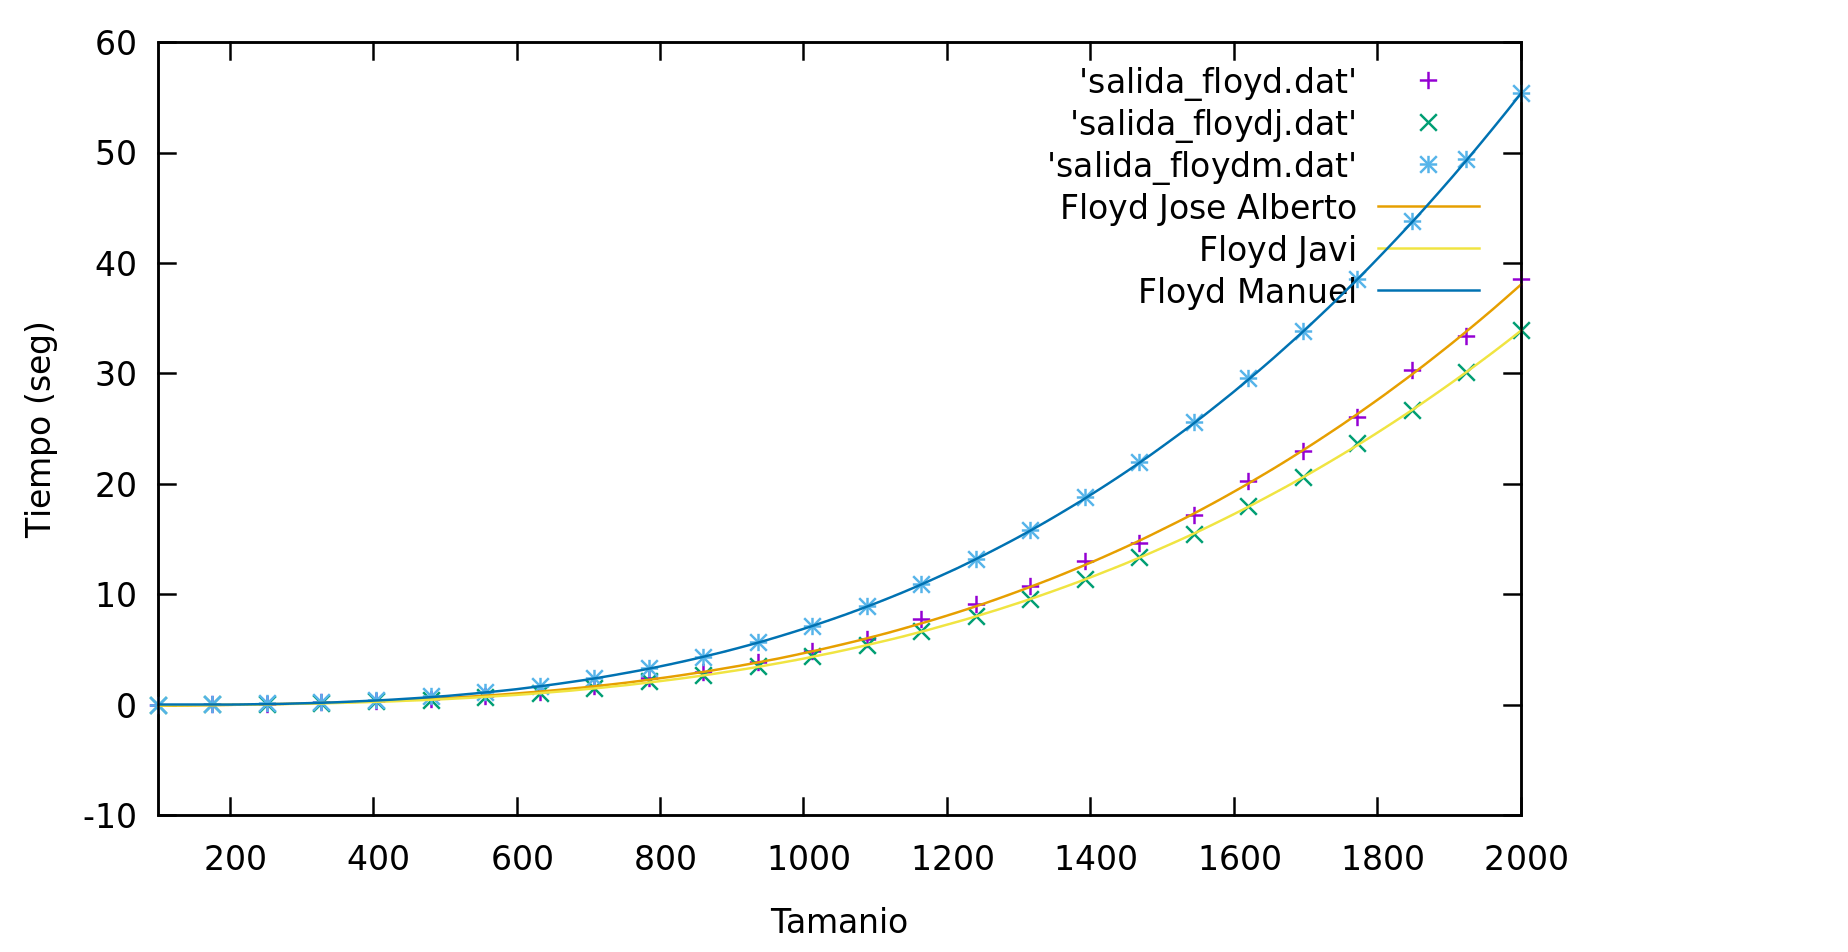
\includegraphics[scale=0.15]{../../Images/floyd_combinados.png}
\end{frame}

\begin{frame}[fragile]{Floyd.
\normalfont{Eficiencia híbrida}}
\begin{itemize}
	\item i7-6700 3.4GHz \(\rightarrow T_1(n) = 4.38237 \cdot 10^{-9} x^3 - 4.33753 \cdot 10^{-7} x^2 + 0.000337001x - 0.0504332\)
	\item i5-1095G1 1.00 GHz \(\rightarrow T_2(n) = 5.12922 \cdot 10^{-9} x^3 - 1.11315 \cdot 10^{-6} x^2 + 0.00083571x - 0.134397\)
	\item Ordenador Moya \(\rightarrow T_3(n) = 6.77297 \cdot 10^{-9} x^3 + 5.13099 \cdot 10^{-7} x^2 - 0.000427834 x + 0.0714028\)
\end{itemize}

Varianza residual:
\begin{itemize}
	\item \(T_1 (n) \longrightarrow Var.res = 0.00204522\)
	\item \(T_2 (n) \longrightarrow Var.res = 0.044778\)
	\item \(T_3 (n) \longrightarrow Var.res = 0.000855184\)
\end{itemize}
\end{frame}

\begin{frame}{Hanoi}
El código del algoritmo de las torres de Hanoi es el siguiente:
\lstinputlisting[language=C++]{./Codes/hanoi.cpp}
\end{frame}

\begin{frame}[fragile]{Hanoi.
\normalfont{Eficiencia teórica}}
Estamos ante un algoritmo recursivo, cuya ecuación de recurrencia es:
\[
	T(n) = 2 T(n-1) +1
\]
\[
	(x-2)(x-1) = 0
\]
\[
	T(n) = c_1 \cdot 2^n + c_2
\]

Por tanto:
\[
	T(n) \in \mathcal{O}(2^n)
\]
\end{frame}

\begin{frame}[fragile]{Hanoi.
\normalfont{Eficiencia empírica}}
\begin{table}[h!]
	\centering
	\footnotesize
	\scalebox{0.6}{
		\begin{tabular}{|c|c|}
			\hline
			\multicolumn{2}{|c|}{\textsf{Intel Core i7-6700 3.40 GHz}}
			\\\hline
			\bfseries Elementos (n) & \bfseries Tiempo (s)
			\csvreader{./data/Javi5454/salida_hanoi.csv}{}
			{\\\hline\csvcoli&\csvcolii}
			\\\hline
		\end{tabular}
		}
		\scalebox{0.6}{
		\begin{tabular}{|c|c|}
			\hline
			\multicolumn{2}{|c|}{\textsf{i5-1095G1 1.00 GHz}}
			\\\hline
			\bfseries Elementos (n) & \bfseries Tiempo (s)
			\csvreader{./data/Jota/salida_hanoi.csv}{}
			{\\\hline\csvcoli&\csvcolii}
			\\\hline
			\end{tabular}
			}
		\scalebox{0.6}{
		\begin{tabular}{|c|c|}
			\hline
			\multicolumn{2}{|c|}{\textsf{Ordenador Moya}}
			\\\hline
			\bfseries Elementos (n) & \bfseries Tiempo (s)
			\csvreader{./data/Moya/salida_hanoi.csv}{}
			{\\\hline\csvcoli&\csvcolii}
			\\\hline
		\end{tabular}
		}
		\caption{Experiencia empírica de algoritmo de Hanoi sin optimizar}
\end{table}
\end{frame}

\begin{frame}[fragile]{Hanoi.
\normalfont{Eficiencia híbrida}}
\centering
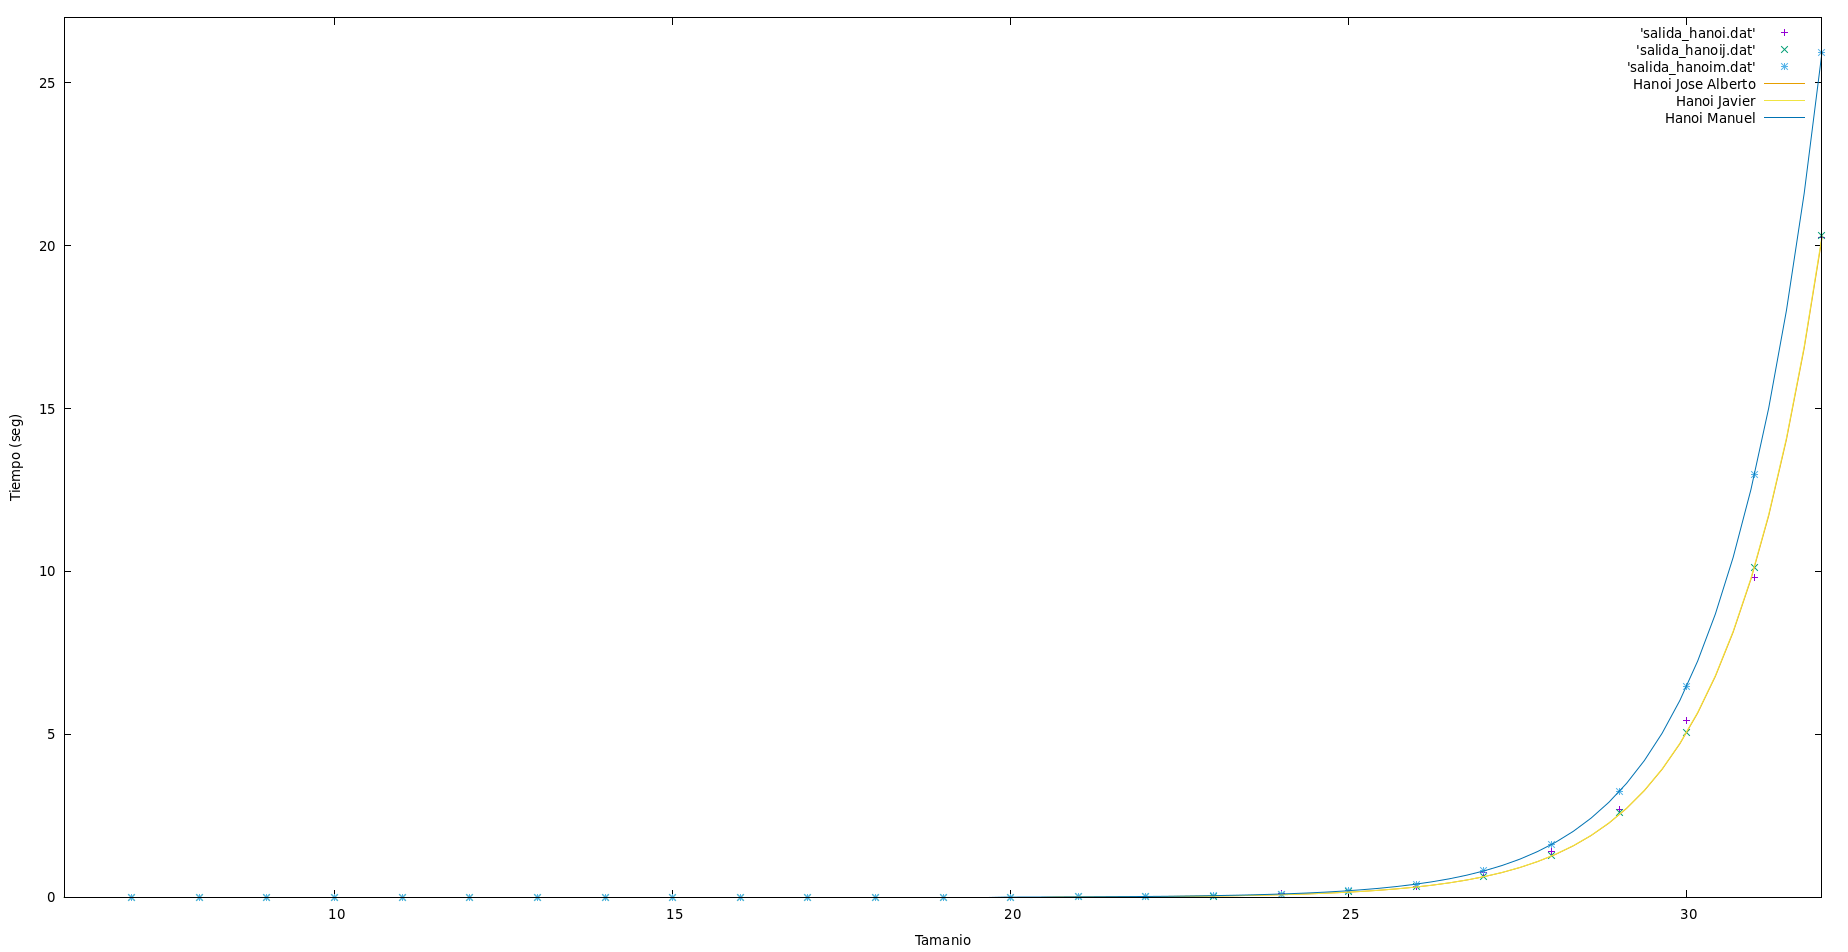
\includegraphics[scale=0.17]{../../Images/hanoi_combinados.png}
\end{frame}

\begin{frame}[fragile]{Hanoi.
\normalfont{Eficiencia híbrida}}
\begin{itemize}
	\item i7-6700 3.40GHz \(\rightarrow T_1(n) = 4.72408 \cdot 10^{-9} \cdot 2^x\).
	\item i5-1095G1 1.00 GHz \(\rightarrow T_2(n) = 4.70707 \cdot 10^{-9} \cdot 2^x\).
	\item Ordenador Moya \(\rightarrow T_3(n) = 6.03512 \cdot 10^{-9} \cdot 2^x\).
\end{itemize}

Varianza residual:
\begin{itemize}
	\item \(T_1(n) \longrightarrow Var.res = 0.000302074\)
	\item \(T_2(n) \longrightarrow Var.res = 0.0113386\)
	\item \(T_3(n) \longrightarrow Var.res = 3.87795 \cdot 10^{-7}\)
\end{itemize}
\end{frame}

\section{Casos especiales}

\begin{frame}[fragile]{Casos especiales.
\normalfont {Floyd Optimizado}}
\centering
\begin{tabular}{cc}
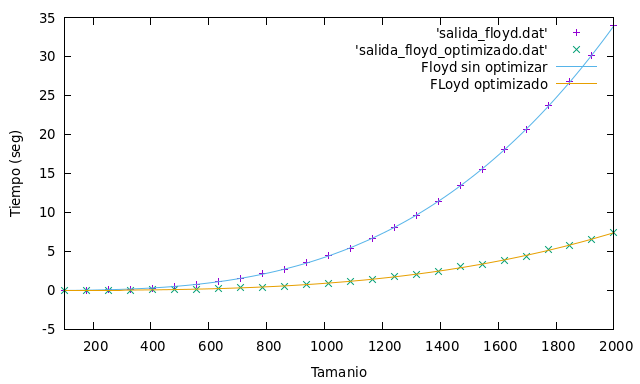
\includegraphics[scale=0.2]{../../Images/floyd_opt_Javi5454.png}
&
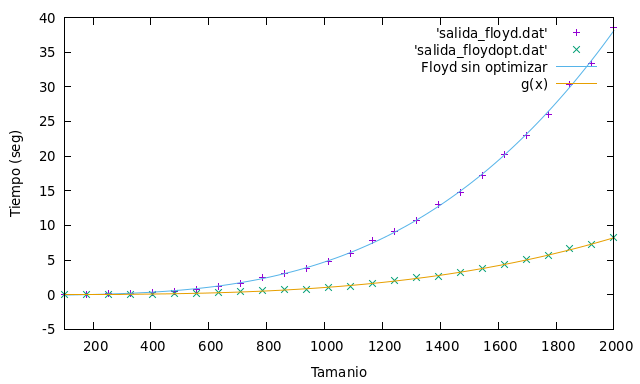
\includegraphics[scale=0.2]{../../Images/floyd_opt_Jota.png}
\\
Intel i7-6700 3.40 GHz & i5-1095G1 1.00 GHz
\end{tabular}
\end{frame}

\begin{frame}[fragile]{Casos especiales.
\normalfont {Otros posibles ajustes funcionales}}
\centering
\begin{tabular}{cc}
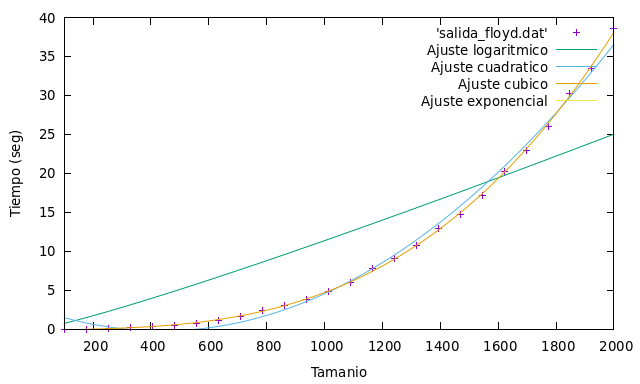
\includegraphics[scale=0.2]{../../Images/floy_comparacion.png}
&
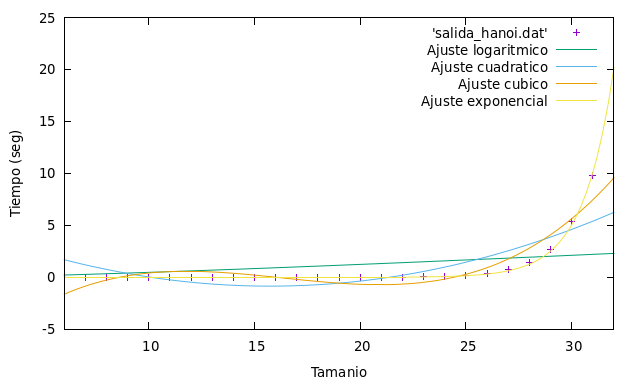
\includegraphics[scale=0.2]{../../Images/hanoi_comparacion.png}
\\
Intel i7-6700 3.40 GHz & i5-1095G1 1.00 GHz
\end{tabular}
\end{frame}


\begin{frame}{Comparativa de los algoritmos de ordenación}
Una vez estudiados inserción, selección, quicksort y heapsort, procedemos a compararlos gráficamente y sacar conclusiones
\end{frame}

\begin{frame}[fragile]{Comparativa de los algoritmos de ordenación}
\centering
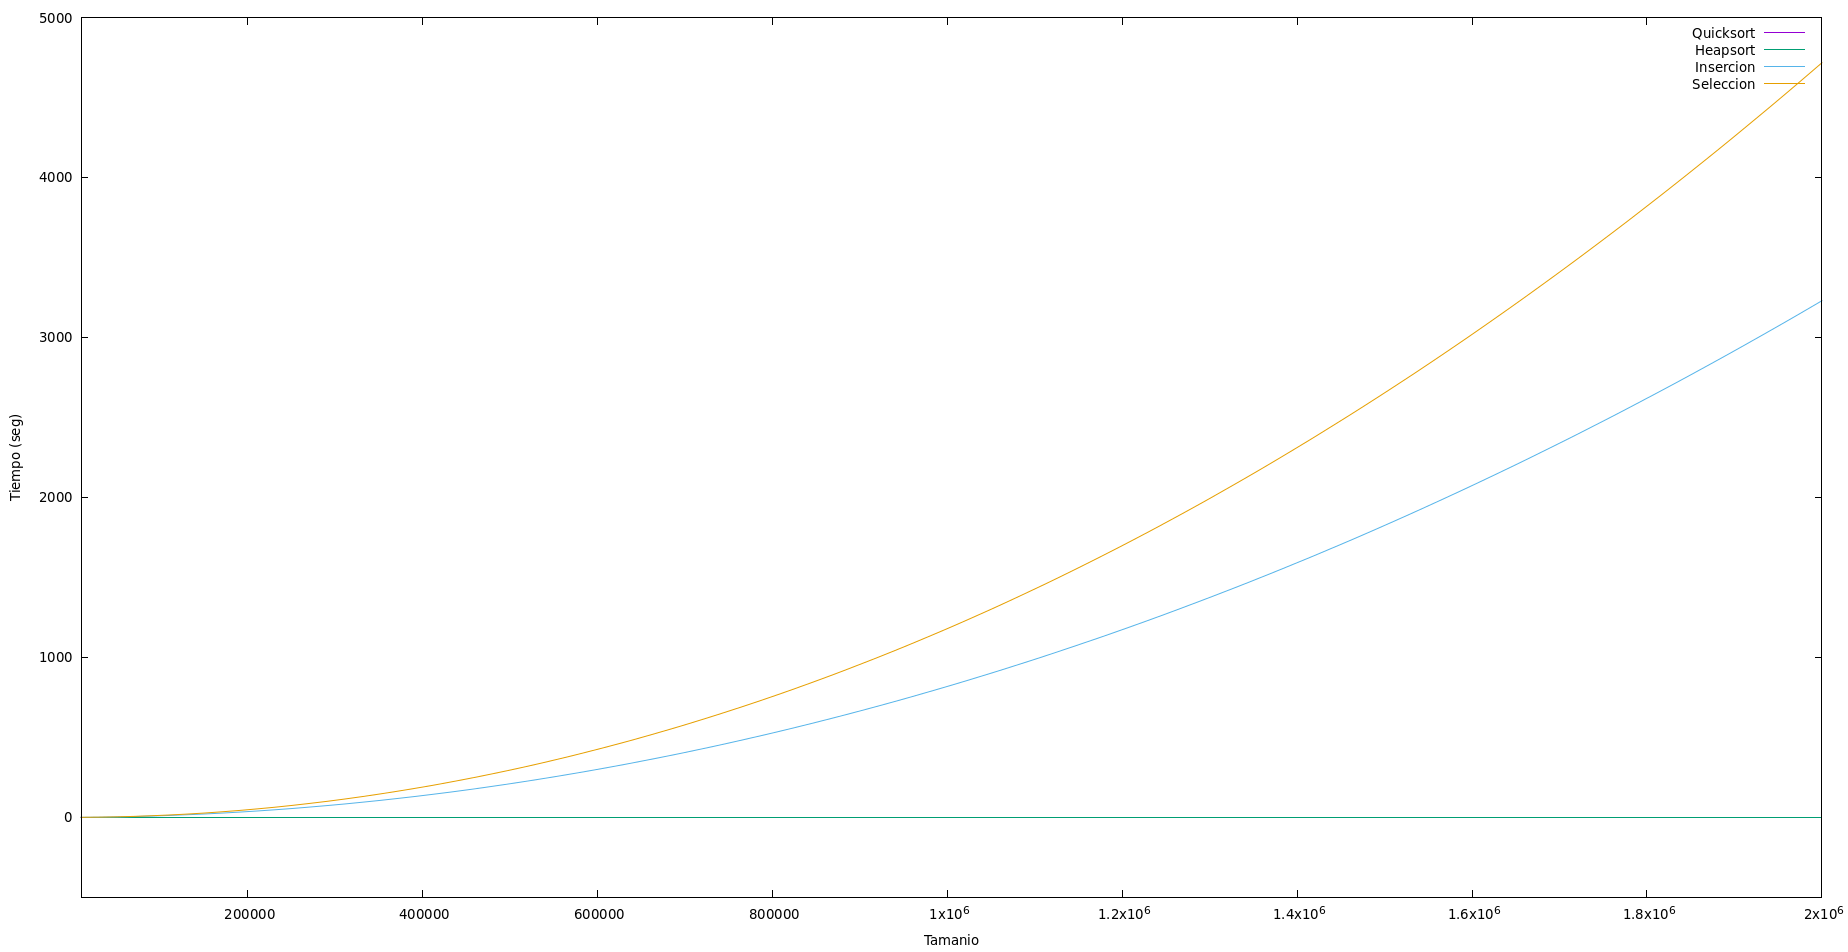
\includegraphics[scale=0.15]{../../Images/Gráfica comparativa algoritmos de ordenación Joshoccas.png}
\end{frame}

\begin{frame}[fragile]{Comparativa de los algoritmos de ordenación}
	\centering
	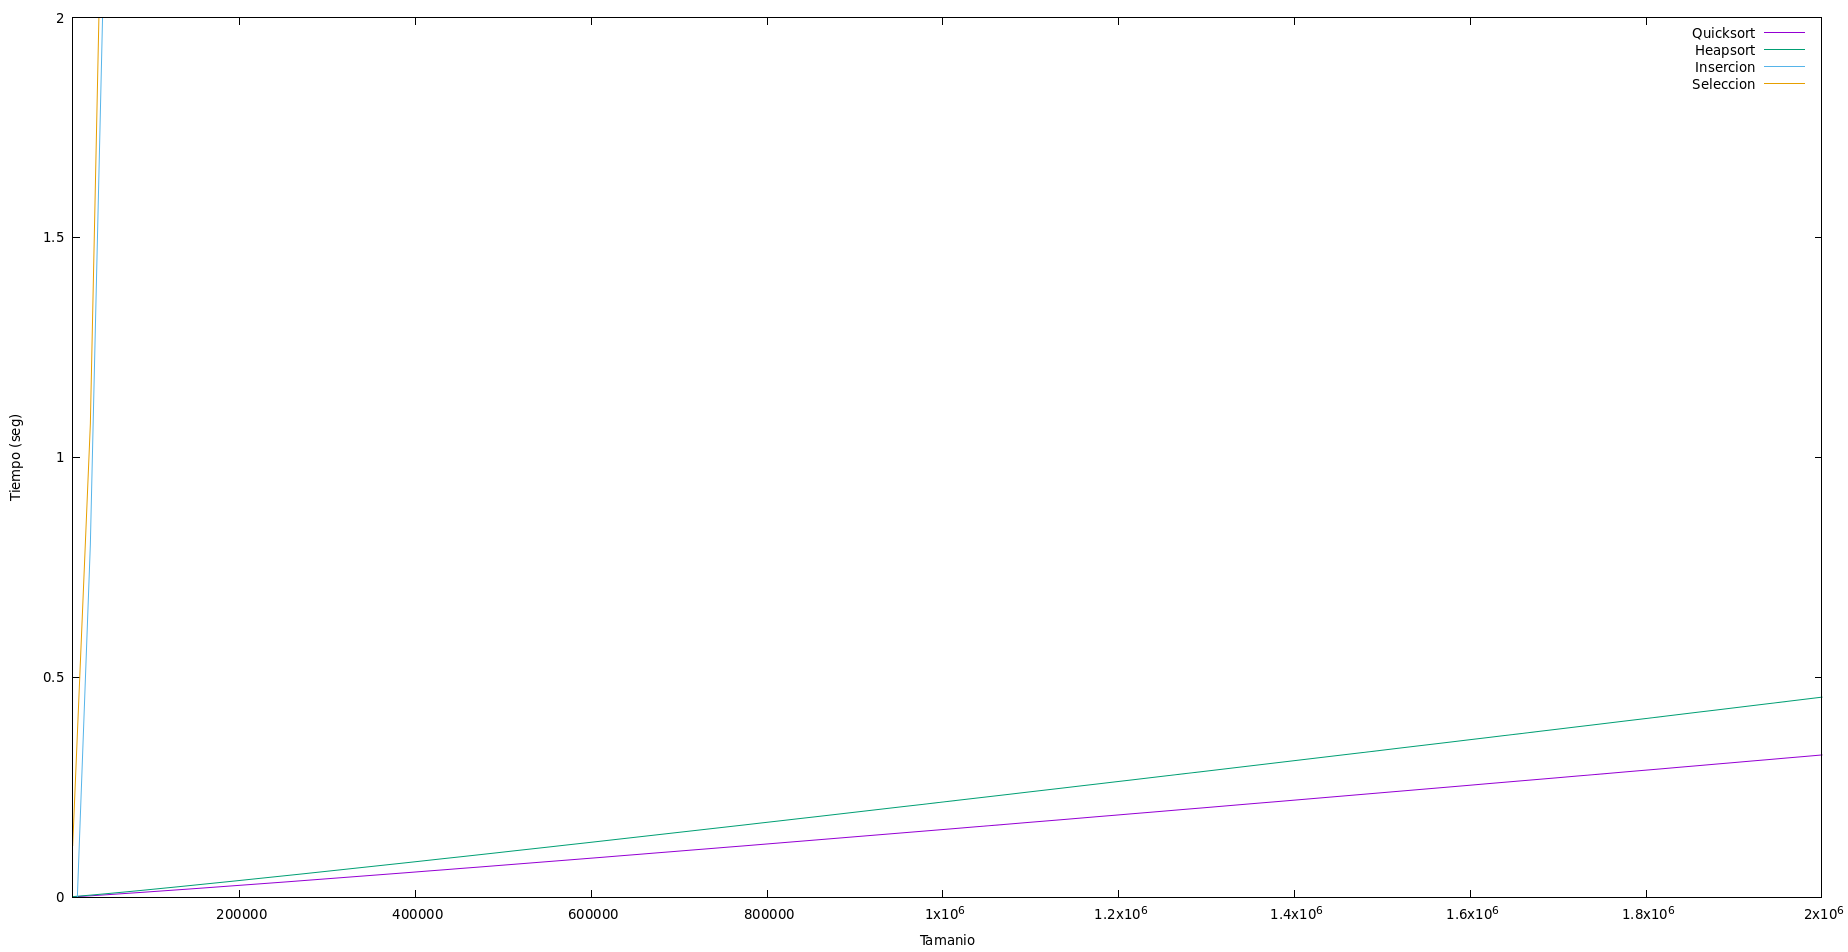
\includegraphics[scale=0.15]{../../Images/Gráfica comparativa algoritmos ordenación Joshoccas (H y Q).png}
\end{frame}

\begin{frame}[fragile]{Comparativa de los algoritmos de ordenación}
Las conclusiones que sacamos son:
\begin{itemize}
	\item Se verifica que los algoritmos \(\in \mathcal{O}(n \cdot log(n))\) son más eficientes que los algoritmos \(\in \mathcal{O}(n^2))\)
	\item Es tal la diferencia que las gráficas de quicksort y heapsort parecen paralelas al eje X
	\item Quicksort y Heapsort no pasan del segundo por ejecución, mientras que Inserción y Selección para 2000000 requieren más de 5000 segundos por ejecución
\end{itemize}
\end{frame}

\begin{frame}{Casos en la ejecución de inserción y selección: 
\normalfont{mejor, peor y promedio}}
	Para el peor caso, tomamos un vector ordenado a la inversa:
	\lstinputlisting[language=Python]{./Codes/peor.cpp}
	Para el mejor caso, tomamos un vector ordenado correctamente:
	\lstinputlisting[language=C++]{./Codes/mejor.cpp}
	
\end{frame}

\begin{frame}{Casos en la ejecución de inserción y selección: 
\normalfont{mejor, peor y promedio}}
Los datasets de los dos casos extremos para inserción fueron:

\begin{table}[h!]
	\centering
	\footnotesize
	\scalebox{0.53}{
		\begin{tabular}{|c|c|}
			\hline
			\multicolumn{2}{|c|}{\textsf{Peor caso de inserción}}
			\\\hline
			\bfseries Elementos (n) & \bfseries Tiempo (s)
			\csvreader{./data/Jota/salida_insercion_peor.csv}{}
			{\\\hline\csvcoli&\csvcolii}
			\\\hline
		\end{tabular}
	}
	\hspace{2cm}
	\scalebox{0.53}{
		\begin{tabular}{|c|c|}
			\hline
			\multicolumn{2}{|c|}{\textsf{Mejor caso de inserción}}
			\\\hline
			\bfseries Elementos (n) & \bfseries Tiempo (s)
			\csvreader{./data/Jota/salida_insercion_mejor.csv}{}
			{\\\hline\csvcoli&\csvcolii}
			\\\hline
		\end{tabular}
	}
\caption{Datasets de la ejecución del peor y mejor caso para Inserción}
\end{table}
\end{frame}

\begin{frame}{Casos en la ejecución de inserción y selección: 
\normalfont{mejor, peor y promedio}}
		\centering
		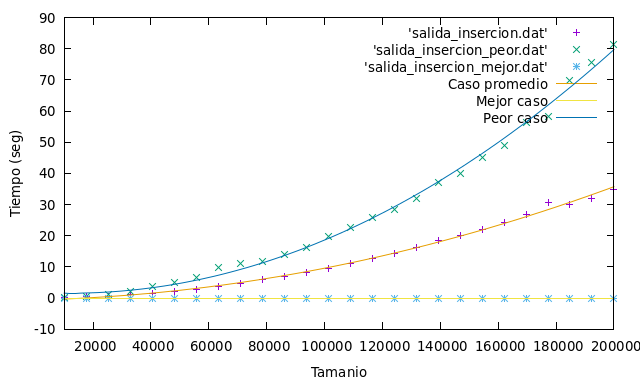
\includegraphics[scale=0.45]{../../Images/Gráfica casos inserción Joshoccas.png}
	\end{frame}

\begin{frame}[fragile]{Casos en la ejecución de inserción y selección: mejor, peor y promedio}
	Los datasets de los dos casos extremos para selección fueron:
	
	\begin{table}[h!]
		\centering
		\footnotesize
		\scalebox{0.53}{
			\begin{tabular}{|c|c|}
				\hline
				\multicolumn{2}{|c|}{\textsf{Peor caso de selección}}
				\\\hline
				\bfseries Elementos (n) & \bfseries Tiempo (s)
				\csvreader{./data/Jota/salida_seleccion_peor.csv}{}
				{\\\hline\csvcoli&\csvcolii}
				\\\hline
			\end{tabular}
		}
		\hspace{2cm}
		\scalebox{0.53}{
			\begin{tabular}{|c|c|}
				\hline
				\multicolumn{2}{|c|}{\textsf{Mejor caso de selección}}
				\\\hline
				\bfseries Elementos (n) & \bfseries Tiempo (s)
				\csvreader{./data/Jota/salida_seleccion_mejor.csv}{}
				{\\\hline\csvcoli&\csvcolii}
				\\\hline
			\end{tabular}
		}
		\caption{Datasets de la ejecución del peor y mejor caso para Selección}
\end{table}
\end{frame}

\begin{frame}[fragile]{Casos en la ejecución de inserción y selección: 
\normalfont{mejor, peor y promedio}}
	\centering
	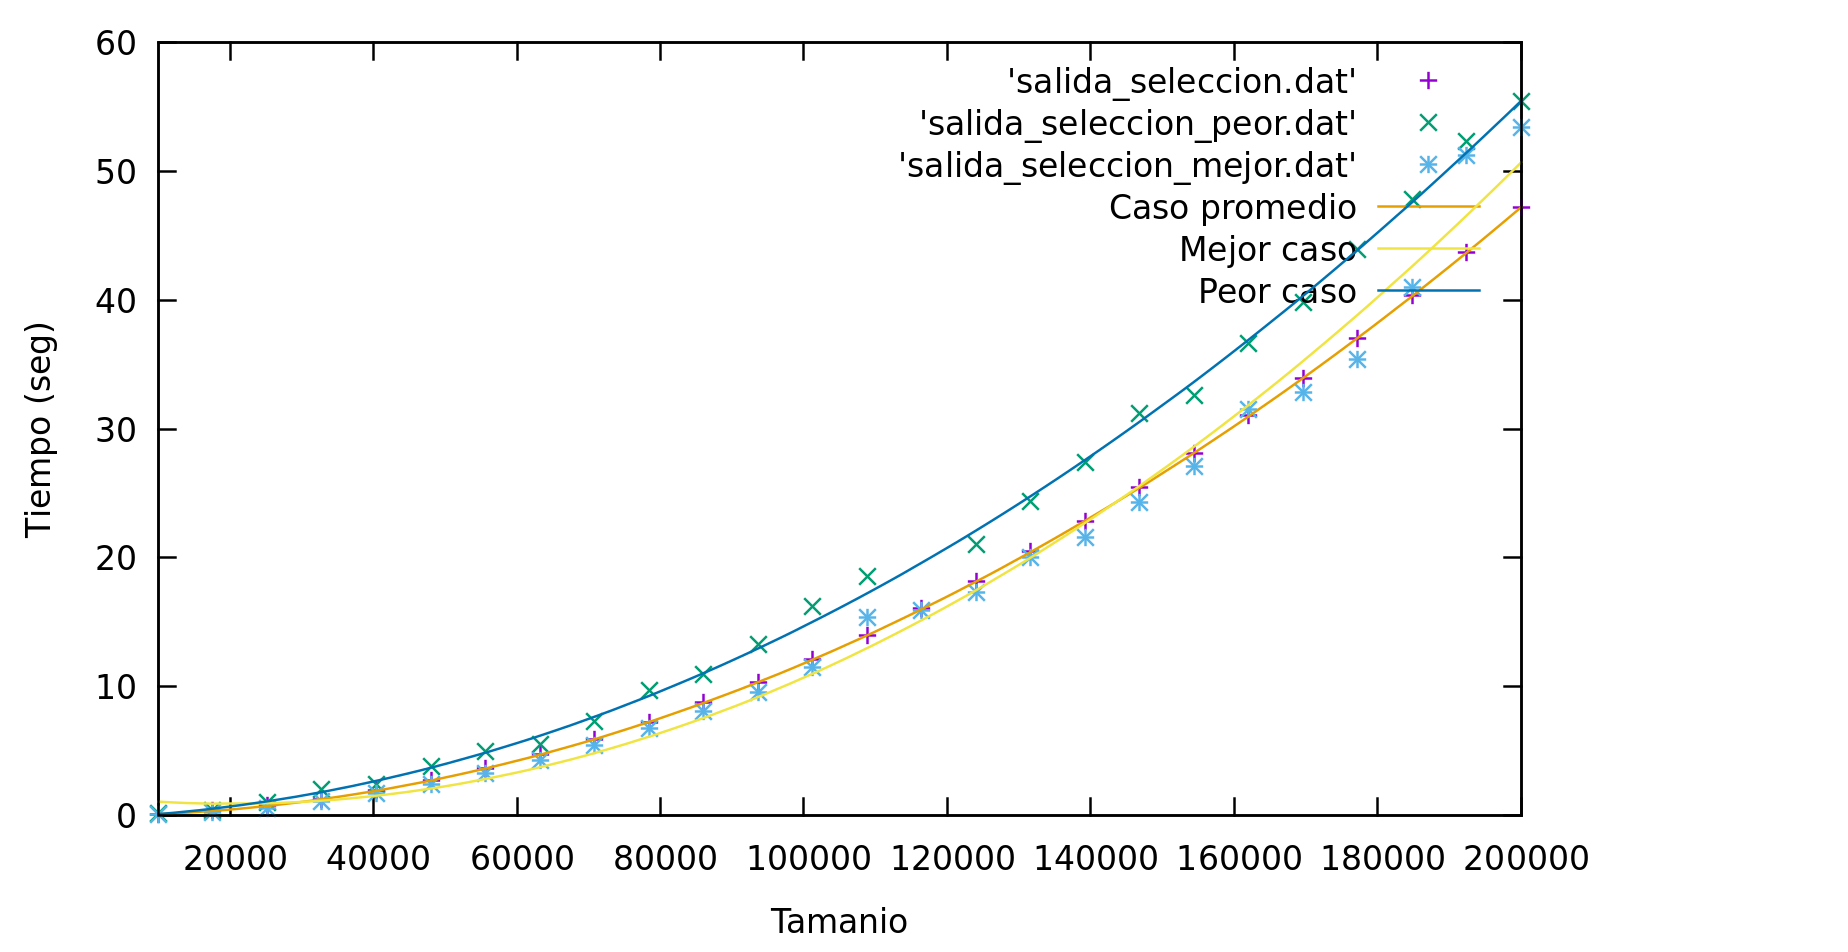
\includegraphics[scale=0.2]{../../Images/Gráfica casos selección Joshoccas.png}
\end{frame}

\begin{frame}[fragile]{Casos en la ejecución de inserción y selección: mejor, peor y promedio}
	\normalfont{¿A qué se debe este comportamiento?}
	\centering
	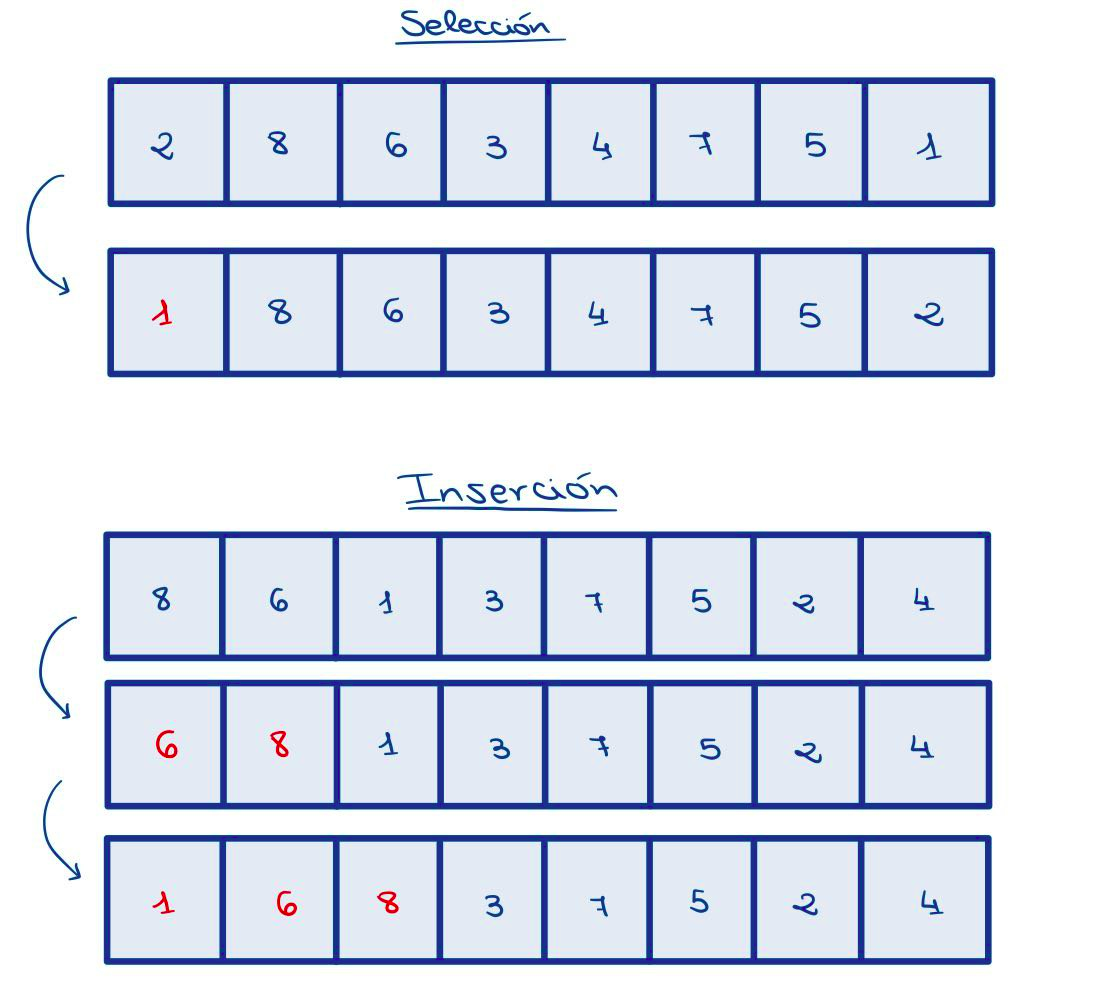
\includegraphics[scale=0.18]{../../Images/Ejemplo vectores.png}
\end{frame}

\section{Conclusiones}

\begin{frame}{Conclusiones}
El análisis híbrido nos confirma nuestro análisis teórico observando el coeficiente de regresión.

Lo que más influye en el tiempo es el orden de eficiencia del algoritmo.

Diversidad de agentes tecnológicos: diferentes computadores y arquitecturas da lugar a resultados distintos.
\end{frame}
\end{document}